\section{Method}
\label{sec:overview}

\begin{figure*}[t]
\centering
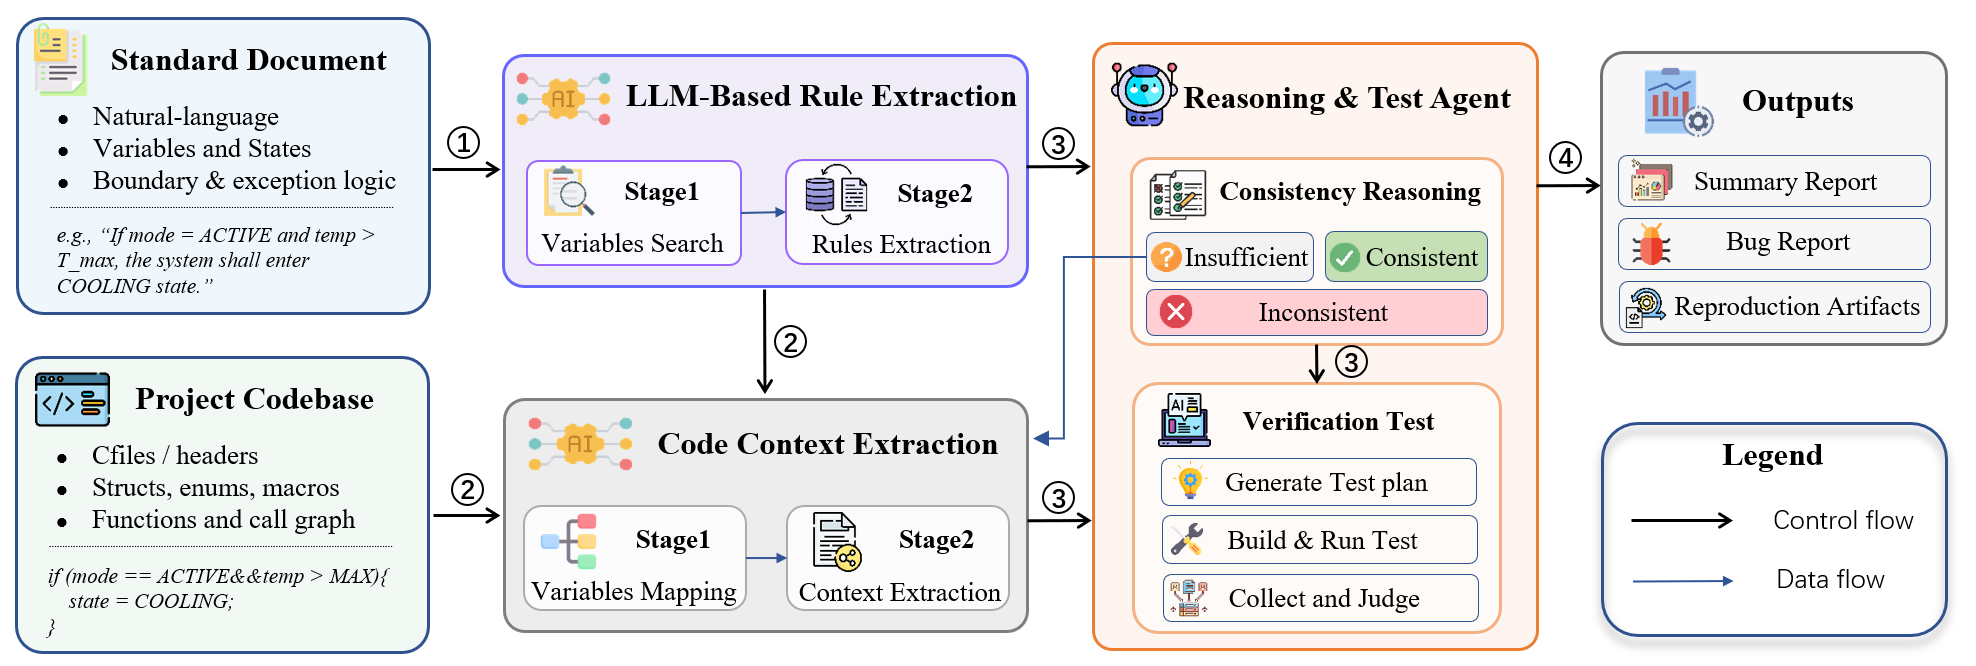
\includegraphics[width=\textwidth]{Figures_1.png}
\caption{Overview of \tool. The original system design has four modules:
standard-document analysis, LLM-based rule extraction, code-context extraction,
and a reasoning-and-test agent that emits summary reports, bug reports, and
reproduction artifacts. Black arrows denote control flow and blue arrows denote
data flow.}
\label{fig:overview}
\end{figure*}

Figure~\ref{fig:overview} shows the \tool{} pipeline. The system takes two
inputs: a natural-language protocol standard and a project codebase. It then
executes three analysis stages before producing outputs: (1) LLM-based rule
extraction from the standard, (2) code-context extraction from the
implementation, and (3) a reasoning-and-test agent that combines both streams of
evidence. The output is not only a label, but a summary report, a bug report,
and reproduction artifacts.

\textbf{Standard-document analysis.}
The left-top input box captures what makes standards hard to analyze:
natural-language requirements, variables and states, and boundary or exception
logic. \tool{} first searches for protocol variables and state-bearing objects,
then extracts field-centric rules from the relevant text. This two-stage design
avoids asking an LLM to directly turn arbitrary prose into bugs.

\textbf{Code-context extraction.}
The left-bottom input box represents implementation evidence: C files, headers,
structures, enums, macros, functions, and call graphs. \tool{} maps each
standard variable to implementation-level identifiers and then extracts the code
contexts needed to evaluate the corresponding rule. This produces the code
evidence consumed by the reasoning agent.

\textbf{Reasoning-and-test agent.}
The agent first performs consistency reasoning and may return
\emph{insufficient}, \emph{consistent}, or \emph{inconsistent}. Insufficient
evidence triggers another code-context extraction round through the blue data
flow edge. For inconsistent or unresolved cases, the verification-test component
generates a test plan, builds and runs the test, and judges the observed
behavior.

\textbf{Reports and artifacts.}
\tool{} produces three classes of outputs: a summary report for triage, a bug
report for maintainers, and reproduction artifacts for validation. This output
structure is central to the paper: the goal is not merely to ask an LLM whether
a rule is violated, but to produce auditable evidence that maintainers can act
on.

\subsection{Design Principles}

\tool{} follows three design principles.

\textbf{Constrain before asking the model.}
The system narrows the problem before each LLM call. Rule extraction is limited
by the field space. Code reasoning is limited by ranked snippets. Test planning
is limited by an explicit defect hypothesis. This structure is intended to
preserve the model's semantic flexibility while reducing opportunities for
ungrounded claims.

\textbf{Prefer evidence over verdicts.}
Every stage emits evidence, not just a label. The rule extractor cites source
spans, the aligner records why a variable was selected, the reasoner cites code
snippets, and the test agent records commands and logs. This evidence-first
style is essential for top-tier review because a detected conformance issue is
only convincing if readers can trace it from standard text to implementation
behavior.

\textbf{Treat uncertainty as progress.}
Many true bugs initially look like missing context, and many false positives
initially look like missing checks. \tool{} therefore treats uncertainty as a
structured intermediate result. A report can remain unresolved with a precise
reason, such as a missing macro definition or an unreachable callback. This
prevents the framework from inflating its bug count by converting every unknown
into an inconsistency.

\subsection{End-to-End Walkthrough}
\label{sec:walkthrough}

This section illustrates the end-to-end behavior of \tool{} using a simplified
transport-parameter example. The purpose is to make the data transformations
concrete before presenting the full implementation details.

\subsubsection{From Standard Text to a Rule}

Suppose a transport standard states that an endpoint receiving a parameter
below a specified lower bound must treat the message as a protocol error. The
sentence is not enough by itself. The checker must know which field is
constrained, which condition activates the rule, what behavior is required, and
where the requirement appears in the document. \tool{} first resolves the
parameter mention against the field space:
\[
\begin{aligned}
C &: \textit{parameter is present in peer transport parameters},\\
f &: \textit{max\_udp\_payload\_size},\\
A &: \textit{reject values below 1200 with a protocol error},\\
M &: \textit{MUST}.
\end{aligned}
\]
The rule retains the original sentence and section number. If another section
defines the bound or error code, that section is attached as a dependency.

\subsubsection{From Rule to Code Evidence}

The aligner expands the field name into aliases such as
\texttt{max\_udp\_payload\_size}, \texttt{max\_payload}, and
\texttt{udp\_payload}. Exact matches alone are insufficient: one file may define
the transport-parameter identifier, another may parse the integer, and a third
may validate the configured connection state. \tool{} therefore retrieves a
bundle containing the parser assignment, the validation helper, and the error
return path. Each snippet is tagged with why it was selected: exact field hit,
symbol scope, action-token overlap, or caller expansion.

\subsubsection{From Evidence to a Judgment}

In the first reasoning round, the model sees the assignment but not the caller
that checks the helper's return value. A one-shot checker may incorrectly report
a missing rejection path. \tool{} instead emits \textsc{Insufficient} with a
typed request for callers of the validation helper. In the second round, the
caller evidence shows that the error return is propagated to connection close.
The final label becomes \textsc{Consistent}. In a different implementation, the
second round might show that the lower-bound check is absent while nearby
upper-bound checks are present, yielding a defect hypothesis.

\subsubsection{From Hypothesis to Validation}

For a suspected mismatch, the validation agent constructs a parameter block
whose value violates the lower bound. It then chooses the closest available
entry point: a unit-test parser if one exists, otherwise a small harness around
the parser function, otherwise a command-line or integration test. The oracle is
derived from the rule: the implementation should reject the input with the
specified protocol error. The final report records the input, command line,
build options, observed return value, and log excerpt. If the harness cannot
reach the relevant path, the report remains unresolved rather than confirmed.

This walkthrough highlights the main difference between \tool{} and direct LLM
inspection. The model is never asked to solve the entire problem from a large
prompt. It receives a constrained rule, a small evidence bundle, and an explicit
choice to request more evidence when the bundle is incomplete.
